\documentclass[class=article, crop=false]{standalone}
\usepackage[subpreambles=true]{standalone}

\usepackage{preamble}

\begin{document}

\begin{center}
    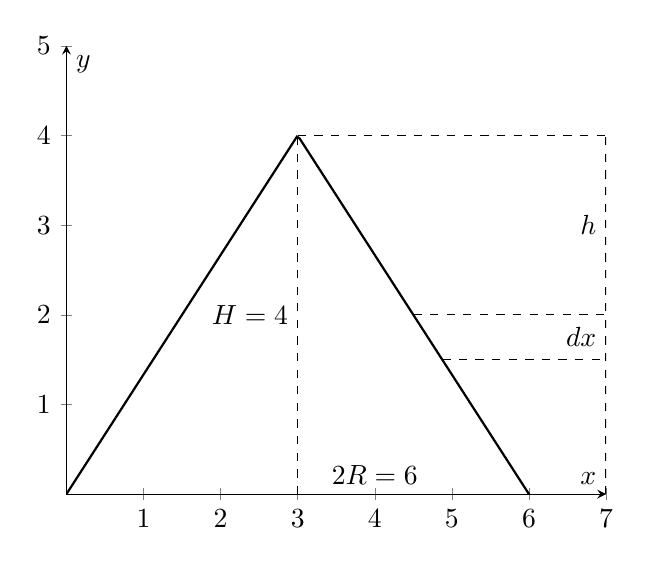
\begin{tikzpicture}
    \begin{axis}[
        xlabel=$x$,
        ylabel={$y$},
        domain=0:7,
        samples=200,
        axis lines=middle,
        ymin=0,
        ymax=5
    ]
    \addplot[thick, color=black] {-abs((4/3)*(x-3))+4};
    \addplot [dashed] coordinates {(3,0) (3,4)};
    \addplot [dashed] coordinates {(7,0) (7,4)};
    \addplot [dashed] coordinates {(3,4) (7,4)};
    \addplot [dashed] coordinates {(4.5,2) (7,2)};
    \addplot [dashed] coordinates {(4.875,1.5) (7,1.5)};
    \node [left] at (axis cs:7,3) {$h$};
    \node [left] at (axis cs:7,1.75) {$dx$};
    \node [above] at (axis cs:4,0) {$2R = 6$};
    \node [left] at (axis cs:3,2) {$H = 4$};
    \end{axis}
    \end{tikzpicture}
    
    \caption{Лемниската Бернулли}
    \label{fig:task4}
\end{center}
\subsubsection*{Ход работы}

\begin{enumerate}
    \item Выделим на конусе малый участок шириной $dh$, верхняя граница которого находится на расстоянии $r$ от плоскости, проходящей через вершину конуса. 

    \item Масса вычисляется по формуле ($m = pV$), где ($p = h^2$) по условию, где $h$ - расстояние от точки на конусе до плоскости.

    \item Можно считать, что плотность на всем выбранном участке одинакова, так как изменение расстояния r будет незначительным. Поэтому массу элементарного участка можно вычислить по формуле ($dm = h^2dV$)

    \item Вычислим объем элементарного учатска конуса. Ввиду его малости, мы можем считать его цилиндром с высотой $dx$, и радиусом основания = $r$.

    \item Из подобия цилиндров следует : $\frac{r}{R} = \frac{h}{H} \Leftrightarrow r = \frac{Rh}{H}$

    \item Объем элементарного участка равен соответственно:

\begin{dmath}
dV = 
2 \cdot \pi \cdot r^2 \cdot dh \Rightarrow dm = 
h^2 \cdot dV = 
h^2 \cdot 2 \cdot \pi \cdot r^2 \cdot dh = 
h^2 \cdot 2 \cdot \pi \cdot (Rh/H)^2 \cdot dh
\end{dmath}

\begin{dmath}
m = 
\int\limits_{0}^{H}(2 \cdot \pi \cdot R^2 \cdot h^4 / H^2 * dh) = 
\int\limits_{0}^{4}(2 \cdot \pi \cdot 9 \cdot \frac{h^4}{4} * dh) = 
\pi \cdot \frac{9}{2} \cdot \int\limits_{0}^{4}(h^4dh) = 
\pi \cdot \frac{9}{2} \cdot \left(\frac{h^5}{5}\right) \Bigg|_{0}^{4} = 
\pi \cdot 0,9 \cdot 1024 \approx 2895.2917
\end{dmath}

\end{enumerate}

\subsubsection*{Заключение}

С помощью интегралов можно вычислять физические величины, значение которых меняется по какому-либо функциональному закону.

\newpage

\end{document}